
\chapter{Simulaciones del modelo microscópico}
\label{cap:simulaciones}

A lo largo de este capítulo describiremos en detalle las simulaciones realizadas sobre el modelo descrito en la Sección \ref{sec:modelo}, en el que se han realizado algunas simplificaciones para facilitar la exposición. En concreto, estudiaremos el comportamiento individual de cada célula y describiremos el resultado global de las decisiones individuales de cada una de ellas. Como ya se ha comentado en el capítulo anterior, es posible ajustar los parámetros del modelo de manera que se  pongan de manifiesto distintos comportamientos poblacionales. Concretamente se presentarán situaciones de tolerancia al \textit{patógeno}, correspondientes al caso en el que las células T no consiguen controlar la infección y el agente que la produce se hace con el control del organismo, situaciones de intolerancia, aquellas en las que las células T terminan con la población de \textit{patógeno}, acabando así con la infección. Se discutirá también qué ocurre cuando  poblaciones de células T con distinta afinidad a un \textit{patógeno} se enfrentan a él.

Además, en este capítulo se exponen algunos detalles básicos sobre la implementación de los algoritmos utilizados para las simulaciones. Entre estas explicaciones se incluye un pseudocódigo y aclaraciones concretas del código. La versión completa del código principal de este capítulo, realizado en Matlab, puede verse en el Apéndice \ref{Appendix:A}. 
 

\section{Modelo simplificado}

Para las simulaciones hemos optado por una versión simplificada del modelo propuesto en la Sección \ref{sec:modelo}, de tal manera que el número de parámetros sea suficiente para no perder la esencia del argumento pero no muy elevado para evitar distraer al lector con notación engorrosa. Siguiendo con la notación de \ref{sec:modelo}, asumiremos $k=2$. Es decir, suponemos que hay dos tipos de receptores en la membrana de nuestras células T: \textit{p} (de proliferación) y \textit{d} (de muerte) que controlan la evolución de los inhibidores de ciclo (Rb) y apoptosis (Bcl-2), respectivamente.

Para las células T efectoras que no forman parte de las células T de memoria (veremos ecuaciones específicas para esta población) asumimos que los receptores de proliferación (\textit{p}) se expresan a partir de las señales que reciben gracias a su TCR y que, simultáneamente, autorregulan su expresión induciendo la producción de receptores tipo muerte (\textit{d}). En este caso, las ecuaciones \ref{sist_inhib} y \ref{sist_recep} pueden escribirse como:

\begin{equation}
	\label{sist9_simplif}
	\left\{ \begin{array}{l}
	\dot{c}(t) = -\mu_{pc}p(t) \\
	\dot{a}(t) = -\mu_{da}d(t)  \\
	\dot{p}(t) = \lambda_{Tp}r_{T}(t) - \lambda_{pp}p(t) \\
	\dot{d}(t) = \lambda_{pd}p(t) \\
	\\
	c(0)=c_0 \\
	a(0)=a_0 \\
	p(0)=p_0 \\
	d(0)=d_0 
	\end{array}
	\right.
\end{equation}

%Así mismo, hemos simulado este Sistema \ref{sist9_simplif} y la Ecuación \ref{sist_pat_T} 
Para el caso de las células T de memoria hay que tener en cuenta que este tipo de células no muere durante la \textit{contracción clonal}, es por ello que las ecuaciones que regulan esta población difieren ligeramente de las vistas en el Sistema \ref{sist9_simplif}. La dinámica de las células T de memoria viene dada por el mismo Sistema \ref{sist9_simplif}, en el que se ha tenido en cuenta que $d=0$, puesto que nos centramos solamente en el inhibidor del ciclo celular y no en el de muerte. Así las cosas, las ecuaciones que rigen el algoritmo de decisión para células T de memoria viene dado por: 

\begin{equation}
	\label{sist15_simplif}
	\left\{ \begin{array}{l}
	\dot{c}(t) = -\mu_{pc}p(t) \\
	\dot{p}(t) = \lambda_{Tp}r_{T}(t) - \lambda_{pp}p(t) \\
	\\
	c(0)=c_0 \\
	p(0)=p_0 \\
	\end{array}
	\right.
\end{equation}

Con estos tres sistemas de ecuaciones (\ref{sist_pat_T}, \ref{sist9_simplif} y \ref{sist15_simplif}) queda definido el marco teórico del modelo. Sin embargo, antes de poder simular numéricamente estas ecuaciones debemos elegir los valores concretos que tomarán los parámetros. Esta no es una tarea sencilla, puesto que nadie sabe cuánto pueden valer estos parámetros en la realidad. La elección de los parámetros que hemos hecho para la primera simulación (Sección \ref{sim:intoler}) se recoge en la Tabla \ref{tabla:param}. En base a esta elección y a las variantes que se exponen a lo largo de esa sección, obtenemos unos resultados que nos permiten identificar distintos tipos de respuesta inmune, sin necesidad de invocar ningún mecanismo distinto a las hipótesis detalladas en la Sección \ref{sec:hip_bio}. A continuación se presentan los detalles básicos de la implementación.


\section{Detalles de implementación y pseudocódigo}

Con ánimo de aclarar algunos aspectos técnicos, se desarrollan, paso por paso, las instrucciones seguidas para la realización de las simulaciones. El Algoritmo \ref{algo:pseudocodigo} contiene un pseudocódigo muy sencillo con los detalles claves y prácticamente independientes del lenguaje de programación que se utilice. El código completo, realizado en Matlab, puede verse en el Apéndice \ref{Appendix:A}.

La población de células T se guarda en una matriz, donde se especifica el tipo de la célula (efectora o de memoria), la cantidad de Rb y Bcl-2 que tiene disponible a su alrededor, el número de receptores de membrana que tiene, la fase en la que se encuentra (división, apoptosis o decisión) y el tiempo que le queda para finalizar la fase correspondiente. Como se trata de un modelo microscópico, en el que cada célula toma su decisión de manera independiente, el hilo conductor de la implementación se basa en recorrer la matriz de células y ejecutar la decisión tomada por la célula que se esté tratando. Cada vez que se recorre la población de células T asumimos que pasa un tiempo $t_{next}$ que actualiza el tiempo actual de la simulación al final de la iteración y que permite determinar cuándo una célula ha acabado la fase de división o apoptosis. Veamos, paso por paso, las instrucciones concretas del modelo.

\begin{enumerate}
	\item Comenzamos la simulación en un tiempo inicial $t=0$ y acabamos en un tiempo final $T_{final}$ que se establecerá una vez las células T efectoras han desaparecido. 
	
	\item Para cada tiempo $t$, se calcula la cantidad de \textit{patógeno} disponible, $Y$. 
	
	\item En función de $Y$, y para cada célula T de la población, se calcula la cantidad de \textit{patógeno} que está a su alcance y se resuelve el sistema de ecuaciones correspondiente para conocer la cantidad de Rb ($c$) y Bcl-2 ($a$) activa en ese instante. En función de esto se desencadenará la división celular, si $c = 0$, o el suicidio de la célula, si $a = 0$. En otro caso la célula seguirá en fase de decisión y volverá a calcular $a$ y $c$ en la siguiente iteración en base a la cantidad obtenida en la actual.
	
	\item Si la célula va a dividirse se generan dos células hijas con los parámetros correspondientes al TCR, recordemos que la cantidad de receptores de la célula madre se divide entre las dos hijas de manera asimétrica, y los parámetros iniciales, para que pueda comenzar su fase de \textit{decisión}. Se sigue en el paso 6.
	
	\item Si por el contrario la célula comete suicidio, se eliminará de la población. 

	\item Se contempla la siguiente célula de la población y se vuelve a 3.
	
	\item Se actualiza el tiempo para la siguiente iteración y se vuelve a 1.
\end{enumerate}


\begin{algorithm}
	\caption{Algoritmo de la decisión. Células T.}
	\label{algo:pseudocodigo}
	\begin{algorithmic}[1]
		
		% ENTRADA / SALIDA
		
		\State Inicialización de parámetros según \ref{tabla:param}
		\State $t = 0;$ \Comment{t será el tiempo por el que vamos simulando}
		
		\While{ $t\ < \ T_{final}$}
		  
		\State $Y = Y_{init}*e^{t*(\alpha - N*\beta)};$ \Comment{Calculamos Y con la solución explícita de \ref{sist_pat_T}}
		
		\For{$nCell; nCell++; N$} \Comment{Para cada célula T de la población}
			\State $ r_{T}=\rho*Y;$ \Comment{Ecuación \ref{ec:rhotau}}
			\If{$efectora(nCell)$} \Comment{Si es una célula T efectora}
				\State Se resuelve \ref{sist9_simplif}
				\If{$a \leq 0 $}
					\State La célula $nCell$ se elimina de la población
				\ElsIf{$c \leq 0$}
					\State La célula $nCell$ se divide
					\State Las condiciones iniciales de las células hijas vienen determinadas por $a_0, c_0$ y \ref{sist:div_sim}
				\EndIf
			
			\ElsIf{$memoria(nCell)$} \Comment{Si es una célula T de memoria}
				\State Se resuelve \ref{sist15_simplif}
				\If{$c \leq 0$}
					\State La célula $nCell$ se divide siguiendo el mismo procedimiento que la división de una célula T efectora. 
				\EndIf
			\EndIf
		\EndFor
		
		\State $t = t + t_{next};$
		\State Se actualiza el número de células de la población.	
		
		\EndWhile
		
	\end{algorithmic}
\end{algorithm}

En este pseudocódigo se ha detallado cuáles son las ecuaciones involucradas en cada paso. A continuación, exponemos algunas particularidades de la simulación: hemos omitido que cuando las condiciones son $a > 0$ y $c > 0$, en el caso de las células T efectoras y $c > 0$, en el caso de las células T de memoria, la célula permanece en la fase de decisión pero actualiza sus condiciones para la siguiente iteración según los resultados que ha obtenido en la iteración actual. También hay que tener en cuenta que la división celular y el proceso de apoptosis no se llevan a cabo de manera inmediata, conllevan un tiempo $t_{cycle}$ y $t_{apo}$, respectivamente, por lo que el número total de células en la población debe actualizarse una vez que estos procesos hayan finalizado y no instantáneamente, como pueden sugerir las líneas $10$, $12$ y $17$. Otro aspecto que hemos supuesto es que el parámetro $\gamma$ que aparecía en la Ecuación \ref{ec:rhotau} es $\gamma = 1$. Es decir, suponemos que todo encuentro del TCR de la célula T con el antígeno va a desencadenar una activación. El parámetro $\rho$ debe ser calculado de tal manera que todas las células T tengan las mismas posibilidades a la hora de \textit{obtener su parte de \textit{patógeno}}, en la implementación real se usó un vector de números aleatorios entre $0$ y $1$ normalizado por el número total de células T. Buena parte de la notación usada en el Algoritmo \ref{algo:pseudocodigo} ya ha sido introducida a lo largo de este trabajo, pero volvemos a insistir en que $Y$ representa el número de moléculas del \textit{patógeno}, mientras que $N$ la cantidad total de células T, incluyendo las efectoras y las de memoria. Sin embargo, en la implementación real, en la línea $4$ del pseudocódigo, el $N$ utilizado es solamente el número total de células T efectoras, sin contar las de memoria\footnote{Esto se ha hecho así porque el proceso que siguen las células T de memoria es más complejo que lo que se recoge en el modelo. Estas células al cabo de un tiempo se desactivan y para que tengan un efecto sobre el \textit{patógeno} deben volver a activarse. Para intentar hacer el modelo lo más sencillo posible se ha optado por hacer que las únicas células que combaten al \textit{patógeno} sean las T efectoras.}.

\section{Resultados y análisis}

En esta sección expondremos los resultados de las simulaciones realizadas. Empezaremos por las dos situaciones básicas que se pueden dar en una infección: que las células inmunes logren controlar la infección o que, por el contrario, sea el agente infeccioso el que acabe tomando el control de nuestro organismo, y acabaremos mostrando el resultado de diversas simulaciones cuando la afinidad por el \textit{patógeno} de las células T va variando.

\subsection{Intolerancia al \textit{patógeno}}
\label{sim:intoler}

La primera de nuestras simulaciones puede verse en la Figura \ref{fig:intolerance}. Se muestra en ella el caso correspondiente a la elección de parámetros que se recoge en la Tabla \ref{tabla:param}. Estamos ante un caso de intolerancia al \textit{patógeno}, puesto que las células T son capaces de controlar la infección eliminarlo por completo. Veámoslo con más detalle: el \textit{patógeno}, representado con un línea roja, crece rápidamente, debido a la elección de una tasa de crecimiento, $\alpha$, elevada. Una vez que las células T son conscientes de la rápida proliferación de un agente no deseado, su número comienza a crecer. Sin embargo, como ya habíamos comentado anteriormente, esto se produce con cierto retraso tras la aparición del \textit{patógeno}. Lo que estamos describiendo es la conocida \textit{expansión clonal}. Este crecimiento de células T provoca que el término que acompaña a $\beta$ en la Ecuación \ref{sist_pat_T} comience a ser más grande que el acompañado por $\alpha$ en esta misma ecuación, provocando así que la derivada de $y$ se haga negativa y, por tanto, el número de moléculas del \textit{patógeno} comience a decrecer. Debemos mencionar que el número de células T necesarias para eliminar el \textit{patógeno} viene regulado por el parámetro $\beta$, si este fuera más grande, es decir, las células T fueran más dañinas con el \textit{patógeno}, el número de células T necesarias para controlar la infección sería menor (y viceversa).

%veríamos una curva azul con un máximo mas pequeño que el de la Figura \ref{fig:intolerance}. (EN REALIDAD EN ESTA FIGURA LA GRÁFICA ESTÁ NORMALIZADA, SERÍA MEJOR PONER LA OTRA SIN NORMALIZAR?)

\begin{table}[h]
	\begin{center}
		\begin{tabular}{>{\centering\arraybackslash}m{2cm} >{\arraybackslash}m{3cm} >{\arraybackslash}m{7cm} }%{|l|l|l|}
			\hline
			\multirow{9}{*}{} & $t_{cycle} = 0.15$               & Duración de la fase de ciclo.                             \\ \cline{2-3}
			& $t_{apo} = 0,2$                  & Duración de la fase de apoptosis.                         \\ \cline{2-3}
			& $t_{next} = 0,3$                 & Duración del paso en la simulación.                       \\ \cline{2-3}
			& $a_0 = 0,3$                      & Cantidad inicial de Bcl-2 para células T efectoras.       \\ \cline{2-3}
			Variables         & $c_0 = 0,08$                     & Cantidad inicial de Rb para células T efectoras.          \\ \cline{2-3}
			& $c_0^{mem} = 0,04$               & Cantidad inicial de Rb para células T de memoria.         \\ \cline{2-3}
			& $N_{ini} = 25$                   & Número inicial de células T naïve.                        \\ \cline{2-3}
			& $Y_{ini} = 5$                    & Número inicial de moléculas del \textit{patógeno}.                 \\ \cline{2-3}
			& $r_p, r_d = 0$                   & Número inicial de receptores de membrana $p$ y $d$.       \\ \hline
			\multirow{2}{*}{Patógeno}  & $\alpha = 6$                    & Tasa de proliferación.                                    \\ \cline{2-3}
			& $\beta = 0,04$                    & Tasa de muerte por linfocito.                             \\ \hline
			\multirow{5}{*}{} & $\lambda_{pd} = 0,05$            & Tasa de cambio del receptor $R_d$ por cada señal $R_p$.   \\ \cline{2-3}
			& $\lambda_{Tp} = 6*10^{-5}$       & Tasa de cambio del receptor $R_p$ por cada señal del TCR. \\ \cline{2-3}
			Células T  efectoras       & $\lambda_{pp} = 0,5*10^{-4}$     & Tasa de cambio del receptor $R_p$ por cada señal $R_p$.   \\ \cline{2-3}
			& $\mu_{pc} = 15$                 & Tasa de cambio de Rb por cada señal del TCR.              \\ \cline{2-3}
			& $\mu_{da} = 10$                 & Tasa de cambio de Bcl-2 por cada señal del TCR.           \\ \hline
			\multirow{4}{*}{} & $\lambda_{Tp}^{mem} = 10^{-5}$   & Igual que $\lambda_{Tp}$, para células T de memoria.      \\ \cline{2-3}
			Células T de memoria        & $\lambda_{pp}^{mem} = 2*10^{-2}$ & Igual que $\lambda_{pp}$, para células T de memoria.      \\ \cline{2-3}
			& $\mu_{pc}^{mem} = 13$           & Igual que $\mu_{pc}$, para células T de memoria.          \\ \cline{2-3}\hline
		\end{tabular}
		\caption{Tabla de variables y parámetros.}
		\label{tabla:param}
	\end{center}
\end{table}


Prestemos atención ahora al comportamiento de las células T de memoria: por la sección anterior, ya sabíamos que las células T efectoras y las de memoria iban a constituir poblaciones distintas, puesto que las ecuaciones que rigen sus dinámicas son distintas. La principal diferencia es que las células T de memoria no se suicidan una vez el \textit{patógeno} ha desaparecido, permanecen con la información necesaria para atacar al \textit{patógeno} más rápidamente en caso de reaparición. En la Figura \ref{fig:intolerance} vemos cómo estas células de memoria aumentan su población tras la aparición del \textit{patógeno}, aunque se produce un crecimiento tan rápido ni elevado como en el caso de las T efectoras. Su población queda reducida a un $5-10\%$ de la población de células T.
%
%\begin{figure}[t]
%	\centering
%	\begin{tabular}{cc}
%		\subfloat[Simulación: caso de intolerancia al \textit{patógeno}. Los parámetros son los expuestos en la Tabla \ref{tabla:param}.]{
%			\label{fig:intolerance}
%			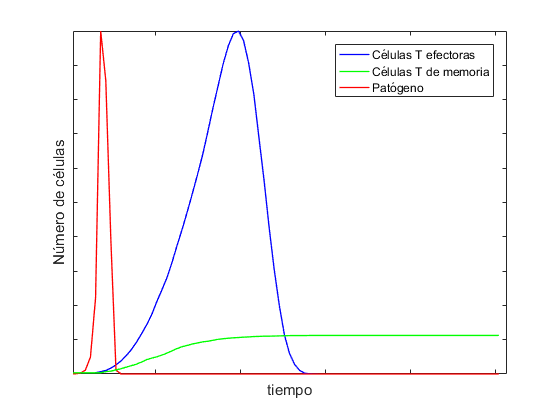
\includegraphics[width=0.5\textwidth]{Imagenes/Simulaciones/intolerance}}
%		& \subfloat[Simulación: caso de tolerancia al \textit{patógeno}. Los parámetros son los mismos que se exponen en la Tabla \ref{tabla:param}, excepto: $\alpha = 1$, $\beta = 0.01$, $\mu_{pc} = 3$, $\mu_{da} = 2$, $\mu_{pc}^{mem} = 2$.]{
%			\label{fig:tolerance}
%			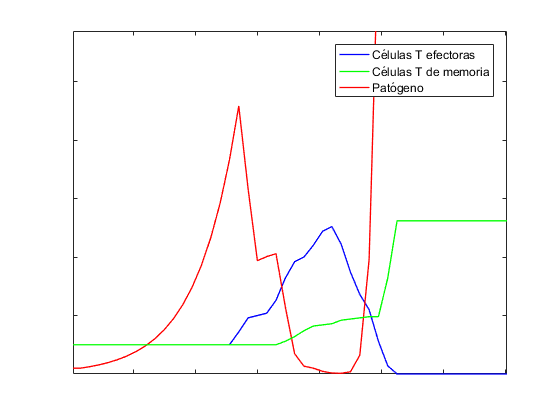
\includegraphics[width=0.5\textwidth]{Imagenes/Simulaciones/tolerance}}\\
%	\end{tabular}
%	\caption{Simulaciones del modelo microscópico. Casos de tolerancia e intolerancia al \textit{patógeno}}%\label{foo}
%\end{figure}

\begin{figure}[t]
	\centering
	%\begin{tabular}{c}
		\subfloat[Simulación: caso de intolerancia al \textit{patógeno}. Los parámetros son los expuestos en la Tabla \ref{tabla:param}.]{
			\label{fig:intolerance}
			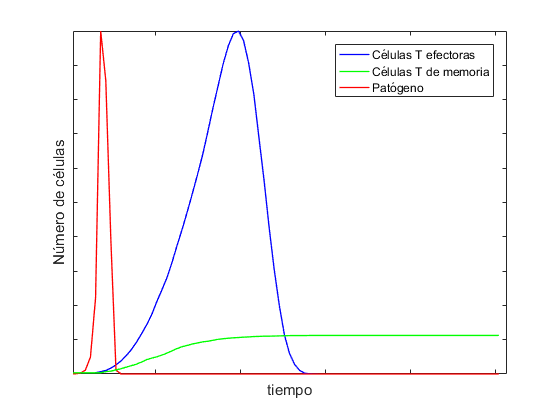
\includegraphics[width=0.7\columnwidth]{Imagenes/Simulaciones/intolerance}}
		
		\subfloat[Simulación: caso de tolerancia al \textit{patógeno}. Los parámetros son los mismos que se exponen en la Tabla \ref{tabla:param}, excepto: $\alpha = 1$, $\beta = 0.01$, $\mu_{pc} = 3$, $\mu_{da} = 2$, $\mu_{pc}^{mem} = 2$.]{
			\label{fig:tolerance}
			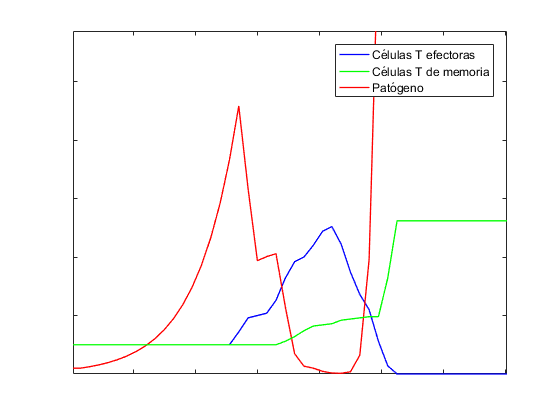
\includegraphics[width=0.7\columnwidth]{Imagenes/Simulaciones/tolerance}}\\
	%\end{tabular}

	\caption{Simulaciones del modelo microscópico. Casos de tolerancia e intolerancia al \textit{patógeno}}%\label{foo}
\end{figure}


%\begin{figure}[t]
%	\centering
%	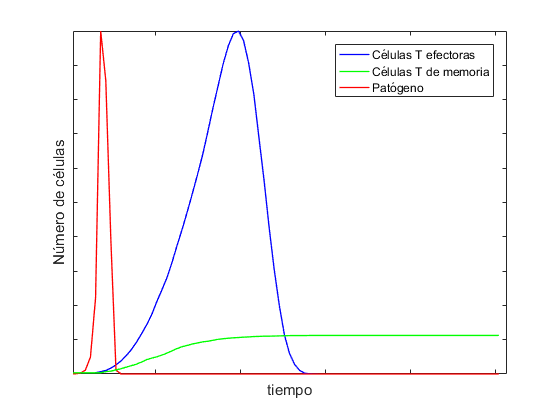
\includegraphics[width=0.7\textwidth]{Imagenes/Simulaciones/intolerance}
%	\caption{Simulación: caso de intolerancia al \textit{patógeno}. Los parámetros son los expuestos en la Tabla \ref{tabla:param}.}
%	\label{fig:intolerance}
%\end{figure}

\subsection{Tolerancia al \textit{patógeno}}
\label{sim:toler}

Hemos visto una simulación de intolerancia al \textit{patógeno}. Esto es, las células inmunes consiguen controlar la infección y erradicar por completo al agente infeccioso. Sin embargo, esto no es siempre así. Existen virus como PONER EJEMPLO SI SE SABE que han desarrollado una estrategia que consiste en crecer a un ritmo muy lento, de esta manera \textit{sigilosa} engañan a las células T, haciéndolas creer que ha sido eliminado y provocando que estas células inmunes se suiciden  \citep{leggett2017growth}. La Figura \ref{fig:tolerance} ilustra esta situación.

Como vemos, las células T comienzan la \textit{expansión clonal} como respuesta a la presencia de \textit{patógeno}, al igual que en el caso anterior. Este aumento de población inmune hace que la población del \textit{patógeno} se vea afectada rápidamente (recordemos que su factor de crecimiento, $\alpha$, es pequeño en este caso) y caiga hasta niveles muy bajos. Es entonces cuando las células inmunes perciben que el \textit{patógeno} ha sido eliminado con éxito y comienzan la \textit{contracción clonal}, haciendo que su población baje hasta desaparecer. Sin embargo, como el \textit{patógeno} no ha sido erradicado por completo y, ahora que no hay atacantes, puede reproducirse sin problema, dando lugar al crecimiento exponencial que vemos en la Figura \ref{fig:tolerance}. En poco tiempo estos \textit{patógenos} \textit{astutos} pueden tomar el control del organismo. 

En cuanto a las células T de memoria, vemos como crecen con la presencia del \textit{patógeno} y se estabilizan cuando la población de células T efectoras llega a cero. Esto es así puesto que las células T de memoria no continúan reproduciéndose en ausencia de células T efectoras, a pesar de la presencia de \textit{patógeno}. PREGUNTAR RAZÓN 

%\begin{figure}[t]
%	\centering
%	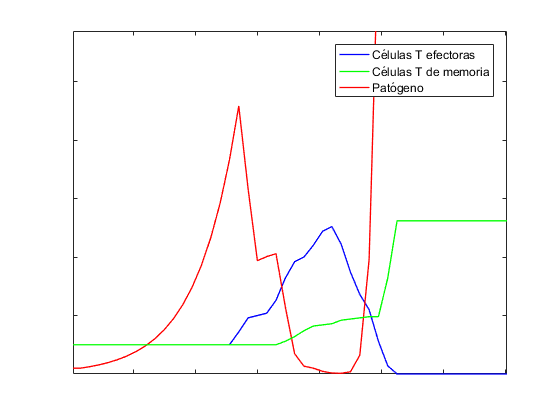
\includegraphics[width=0.7\textwidth]{Imagenes/Simulaciones/tolerance}
%	\caption{Simulación: caso de tolerancia al \textit{patógeno}. Los parámetros son los mismos que se exponen en la Tabla \ref{tabla:param}, excepto: $\alpha = 1$, $\beta = 0.01$, $\mu_{pc} = 3$, $\mu_{da} = 2$, $\mu_{pc}^{mem} = 2$.}
%	\label{fig:tolerance}
%\end{figure}

\subsection{Simulaciones con distintas poblaciones de células T}

En esta sección veremos cómo se comportan distintas poblaciones de células T efectoras frente a un mismo \textit{patógeno}. Estas poblaciones están diseñadas para que tengan afinidades distintas con el \textit{patógeno}. Un caso interesante es ver qué ocurre cuando alguna de estas poblaciones desaparece. 

Comencemos mirando la Figura \ref{fig:tresClones}. En esta simulación hemos considerado tres poblaciones con distinta afinidad, $\lambda_{Tp}$, al \textit{patógeno}. Tenemos el clon $0$ con la afinidad más alta y el clon $2$ con la más baja. La diferencia en cuanto a expansión es considerable, la población más afín al \textit{patógeno} es la que se reproduce a mayor velocidad y se denomina \textit{población inmunodominante}. Este hecho es consecuencia de las ecuaciones del Sistema \ref{sist9_simplif}: la ecuación $\dot{p}(t) = \lambda_{Tp}r_{T}(t) - \lambda_{pp}p(t)$ propicia un mayor crecimiento cuanto más alto es el valor $\lambda_{Tp}$, puesto que provoca que la derivada de $c$ se haga más negativa y se llegue antes al límite $c = 0$ que desencadena la división celular.

%\begin{figure}[t]
%	\centering
%	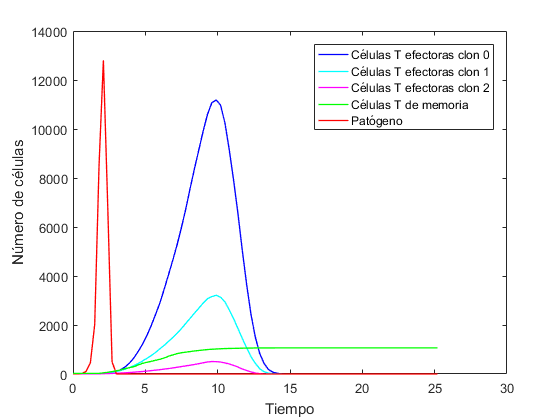
\includegraphics[width=0.7\textwidth]{Imagenes/Simulaciones/tresClones}
%	\caption{Simulación: distintas poblaciones de células T con distintas afinidades al \textit{patógeno}. Los parámetros son los mismos que se exponen en la Tabla \ref{tabla:param}, excepto: $\lambda_{Tp}^{clon_0} = 2*10^{-4}$, $\lambda_{Tp}^{clon_1} = 6*10^{-5}$, $\lambda_{Tp}^{clon_2} = 10^{-5}$.}
%	\label{fig:tresClones}
%\end{figure}


Pero... ¿qué pasaría si esta \textit{población inmunodominante} desapareciera? Una posible explicación nos la da la Figura \ref{fig:dosClones}. En ella, podemos ver que el modelo sugiere que las \textit{poblaciones subdominantes} se expanden más que antes para suplir la ausencia de la \textit{inmunodominante} y controlar la infección. No debemos olvidar que la afinidad que tienen estas poblaciones al \textit{patógeno} es menor y esto hace que pueda crecer más en el mismo periodo de tiempo.


%\begin{figure}[t]
%	\centering
%	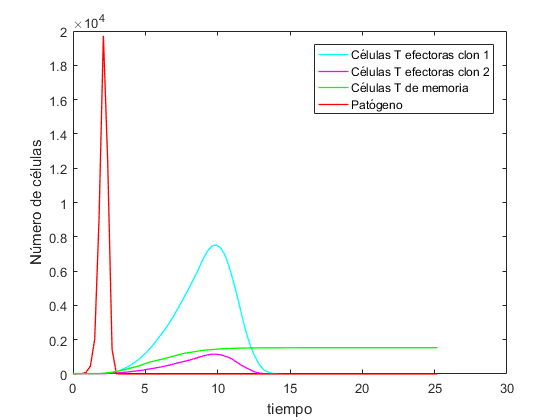
\includegraphics[width=0.7\textwidth]{Imagenes/Simulaciones/dosClones}
%	\caption{Simulación: distintas poblaciones de células T con distintas afinidades al \textit{patógeno}. Clones subdominantes. Los parámetros son los mismos que se exponen en la Tabla \ref{tabla:param}, excepto: $\lambda_{Tp}^{clon_1} = 6*10^{-5}$, $\lambda_{Tp}^{clon_2} = 10^{-5}$.}
%	\label{fig:dosClones}
%\end{figure}

Para finalizar veamos el comportamiento del clon $2$ cuando el resto de clones han desaparecido. Como es de esperar, ocurre algo similar a lo que veíamos en la Figura \ref{fig:dosClones}. En este caso el clon $2$ debe hacer un esfuerzo mayor (reproducirse más) para mantener la infección controlada. Comportamiento ilustrado en la Figura \ref{fig:unClon}.

Estas simulaciones ponen de manifiesto la importancia de las células T de memoria. En una situación donde las células T efectoras no presentan una afinidad al \textit{patógeno} muy elevada las consecuencias pueden ser muy graves, pues la infección se alarga y las células T no son suficientemente dañinas para el agente externo. Sin embargo, si contamos con células T de memoria que guardan información relevante para combatir a ese agente, nuestro organismo se encontrará en una situación más segura, ya que se podrá actuar más rápidamente con células que disponen de alta afinidad con el \textit{patógeno} y desencadenarán, por tanto, un ataque mucho más efectivo.

%\begin{figure}[t]
%	\centering
%	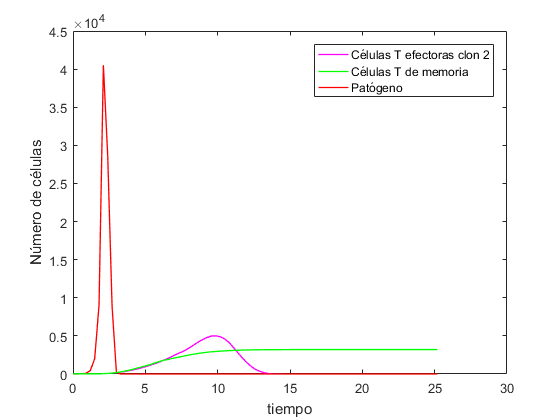
\includegraphics[width=0.7\textwidth]{Imagenes/Simulaciones/unClon}
%	\caption{Simulación: distintas poblaciones de células T con distintas afinidades al \textit{patógeno}. Clon subdominante. Los parámetros son los mismos que se exponen en la Tabla \ref{tabla:param}, excepto: $\lambda_{Tp}^{clon_2} = 10^{-5}$.}
%	\label{fig:unClon}
%\end{figure}


\begin{figure}[t]
	\centering
	%\begin{tabular}{c}
	\subfloat[Simulación: distintas poblaciones de células T con distintas afinidades al \textit{patógeno}. Clones subdominantes. Los parámetros son los mismos que se exponen en la Tabla \ref{tabla:param}, excepto: $\lambda_{Tp}^{clon_1} = 6*10^{-5}$, $\lambda_{Tp}^{clon_2} = 10^{-5}$.]{
		\label{fig:tresClones}
		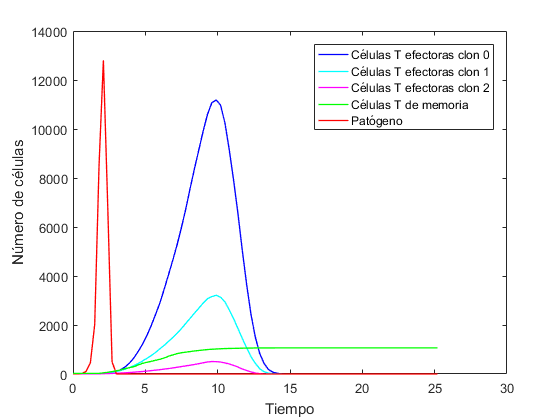
\includegraphics[width=0.5\columnwidth]{Imagenes/Simulaciones/tresClones}}
	
	\subfloat[Simulación: distintas poblaciones de células T con distintas afinidades al \textit{patógeno}. Clones subdominantes. Los parámetros son los mismos que se exponen en la Tabla \ref{tabla:param}, excepto: $\lambda_{Tp}^{clon_1} = 6*10^{-5}$, $\lambda_{Tp}^{clon_2} = 10^{-5}$.]{
		\label{fig:dosClones}
		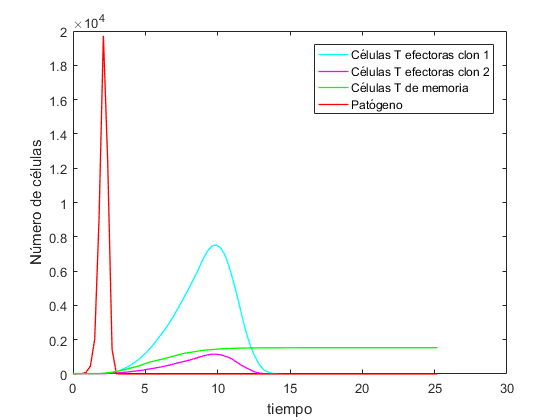
\includegraphics[width=0.5\columnwidth]{Imagenes/Simulaciones/dosClones}}\
	
	\subfloat[Simulación: distintas poblaciones de células T con distintas afinidades al \textit{patógeno}. Clon subdominante. Los parámetros son los mismos que se exponen en la Tabla \ref{tabla:param}, excepto: $\lambda_{Tp}^{clon_2} = 10^{-5}$.]{
		\label{fig:unClon}
		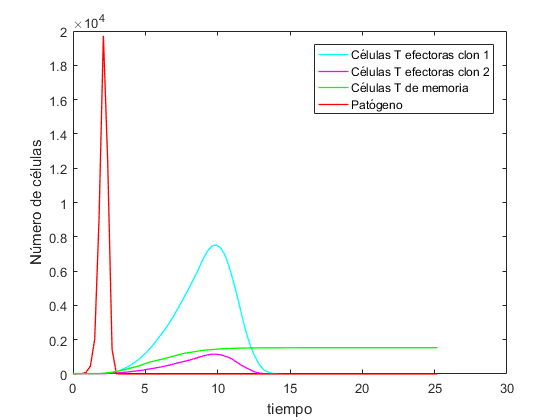
\includegraphics[width=0.5\columnwidth]{Imagenes/Simulaciones/dosClones}}\\
	
	\caption{Simulaciones del modelo microscópico. Casos de tolerancia e intolerancia al \textit{patógeno}}%\label{foo}
\end{figure}
